\documentclass[a4paper, 12pt]{article}

\usepackage{charter}
\usepackage{makeidx}
\usepackage{fancyhdr}
\usepackage{hyperref}
\usepackage[utf8]{inputenc}
\usepackage{graphicx}
\usepackage[left=2cm, right=2cm]{geometry}
\usepackage{latexsym}
\usepackage{amsmath, amsthm, amssymb}
\usepackage{rotating}


\begin{titlepage}
\title{Domain Model}
\author{Release 0.1}
\date{\today \\Firenze \\\begin{figure}[h] \centering

\includegraphics[width=0.2\textwidth]{../../../images/logokiwi.png} 
\end{figure}
}
\end{titlepage}

\pagestyle{fancy}

\begin{document}

\maketitle

\newpage

\section*{Approvazione, redazione, lista distribuzione}
\begin{table}[h!]
  \begin{center}
    \begin{tabular}{| l | l | p{60mm} |}
    \hline
    \textbf{approvato da} & \textbf{il giorno} & \textbf{firma} \\
	\hline    
	Marco Tinacci &  &  \\
    \hline
    \end{tabular}
  \end{center}
\end{table}

\begin{table}[h!]
  \begin{center}
    \begin{tabular}{| l | l | p{60mm} |}
    \hline
    \textbf{redatto da} & \textbf{il giorno} & \textbf{firma} \\
    \hline
    Francesco Calabri &  &  \\
    \hline
	Manuele Paulantonio &  &  \\
    \hline    
	Massimo Nocentini &  &  \\
    \hline
    \end{tabular}
  \end{center}
\end{table}

\begin{table}[h!]
  \begin{center}
    \begin{tabular}{| l | l | p{60mm} |}
    \hline
    \textbf{distribuito a} & \textbf{il giorno} & \textbf{firma} \\
	\hline    
	Daniele Poggi &  &  \\
    \hline
	Niccol\'o Rogai &  &  \\
    \hline
	Marco Tinacci &  &  \\
    \hline
    \end{tabular}
  \end{center}
\end{table}

\newpage

\tableofcontents

\newpage

\section*{Introduzione}

\newpage

\section{Overall diagram}
\begin{figure}[h!] 
	\centering
	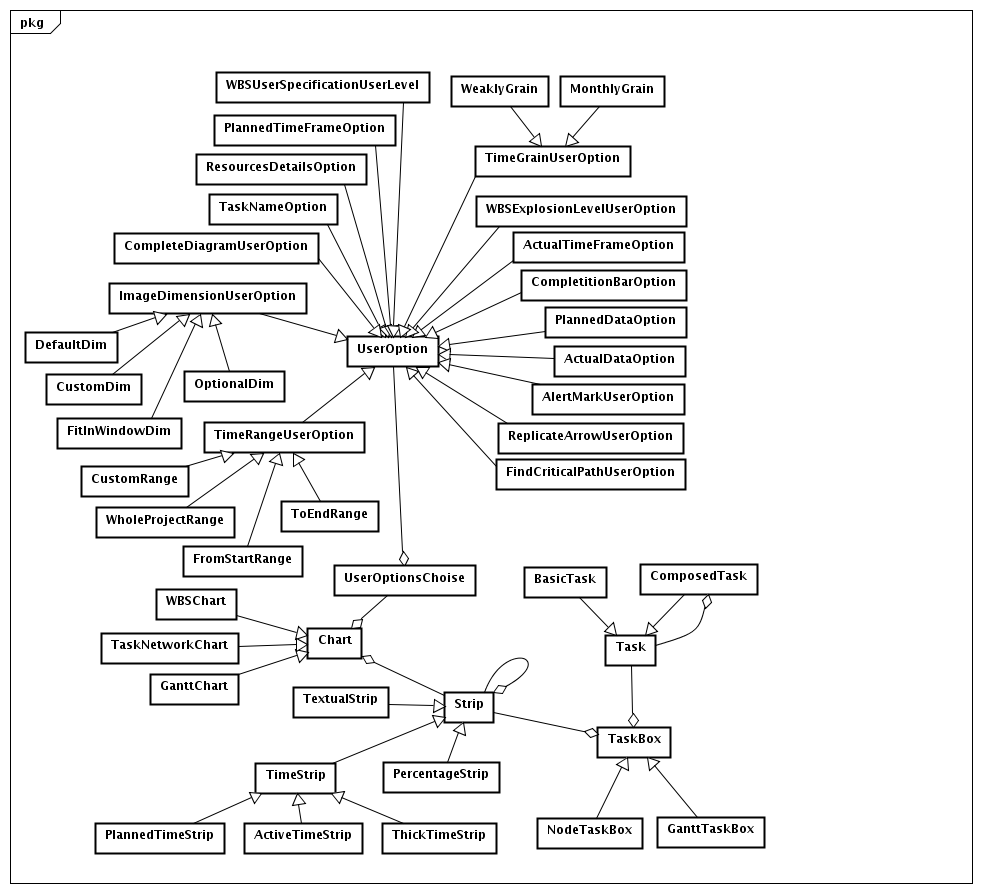
\includegraphics[width=1\textwidth]{../DomainModel.png}
	\caption{Overall UML diagram}
	\label{fig:overallDiagram} 
\end{figure}

\end{document}